%
% `template_basic.tex' - A bare-bones example of using the AIAA class.
%                        For a more advanced usage, see `template_advanced.tex'.
%
% Typical processing for PostScript (PS) output:
%
%  latex template_basic
%  latex template_basic   (repeat as needed to resolve references)
%
%  xdvi template_basic    (onscreen draft display)
%  dvips template_basic   (postscript)
%  gv template_basic.ps   (onscreen display)
%  lpr template_basic.ps  (hardcopy)
%
% With the above, only Encapsulated PostScript (EPS) images can be used.
%
% Typical processing for Portable Document Format (PDF) output:
%
%  pdflatex template_basic
%  pdflatex template_basic      (repeat as needed to resolve references)
%
%  acroread template_basic.pdf  (onscreen display)
%
% If you have EPS figures, you will need to use the epstopdf script
% to convert them to PDF because PDF is a limmited subset of EPS.
% pdflatex accepts a variety of other image formats such as JPG, TIF,
% PNG, and so forth -- check the documentation for your version.
%
% If you do *not* specify suffixes when using the graphicx package's
% \includegraphics command, latex and pdflatex will automatically select
% the appropriate figure format from those available.  This allows you
% to produce PS and PDF output from the same LaTeX source file.
%
% To generate a large format (e.g., 11"x17") PostScript copy for editing
% purposes, use
%
%  dvips -x 1467 -O -0.65in,0.85in -t tabloid template_basic
%
% For further details and support, read the Users Manual, aiaa.pdf.
%
% This software is released under the terms of the LaTeX Project Public
% License.  Copyright (C) 2004 by Bil Kleb, Bill Wood, and Erich Knausenberger.

\documentclass[]{aelab_aiaa-tc}% insert '[draft]' option to show overfull boxes

 \title{Thermodynamic properties of air at high temperature\\
        }

 \author{
  Sanjay V. Gorur
  %\thanksibid{1}\\
  \\{\normalsize\itshape
   Undergraduate student, Aerospace Department, IIST}\\
  \and
  %Third C. Author%
   %\thanks{Job Title, Department, Address, and AIAA Member Grade.}\\
  %{\normalsize\itshape
  %Business or Academic Affiliation, City, Province, Zipcode, Country}
 }

 % Data used by 'handcarry' option if invoked
 \AIAApapernumber{YEAR-NUMBER}
 \AIAAconference{Conference Name, Date, and Location}
 \AIAAcopyright{\AIAAcopyrightD{YEAR}}

 % Define commands to assure consistent treatment throughout document
 \newcommand{\eqnref}[1]{(\ref{#1})}
 \newcommand{\class}[1]{\texttt{#1}}
 \newcommand{\package}[1]{\texttt{#1}}
 \newcommand{\file}[1]{\texttt{#1}}
 \newcommand{\BibTeX}{\textsc{Bib}\TeX}

\begin{document}

\maketitle

%\begin{abstract}
%The goal of this practice session was to determine the actuating torque and reaction forces on links of a shaper mechanism.
%\end{abstract}

%\begin{abstract}
	%The goal of this practice session was to determine the actuating torque and reaction forces on links of a shaper mechanism.
%\end{abstract}

\begin{abstract}
	
	Thermodynamic properties of air are obtained for air at high temperature using the partition function approach in statistical mechanics. The composition of air is simplified to be made up of seven species namely $N_2$, $O_2$, $NO$, $NO^+$,$N$, $O$ and $e^-$. Curve fits are obtained for the specific heat capacity of air at temperatures ranging upto 30000K and presurres varying from 1atm to 90atm.
	
\end{abstract}

\section*{Nomenclature}

\begin{tabbing}
	XXXXXXXXXXXX \= \kill% this line sets tab stop
	$Q$ \> Partition function \\
	$Q_{tr}$ \> Translational partition function \\
	$Q_{int}$ \> Internal partition function \\
	$m$ \> Mass, Kg \\
	$k$ \> Boltzmann constant, SI \\
	$h$ \> Planck's constant, SI \\
	$E_{vib}$ \> Vibrational energy \\
	$E_{rot}$ \> Rotational energy \\
	$\omega_{e}, \omega_{e}x_e, \omega_{e}y_e$ \> Spectroscopic constants - anharmonic oscillator \\
	$c$ \> Speed of light \\
	$D_0$ \> Dissociation energy referenced to first energy level\\
	$D_e$ \> Dissociation energy\\
	$B_\nu, D_\nu$ \> Spectroscopic constants - non-rigid rotator \\
	$\alpha_e, \beta_e$ \> Spectroscopic constants - corrections to rotator \\
	$r_e$ \> Equilibrium distance \\
	$Cp$ \> Specific heat capacity \\
	$Kp$ \> Equilibrium constant of pressure \\
	$p_i$ \> Partial pressure of the ith species \\
	$X_i$ \> Mole fraction of the ith species \\
	$T$ \> Temperature \\[5pt] \\
	
	
	\textit{Subscript}\\
	$i$ \> Variable to denote species \\
\end{tabbing}

\section{Introduction}
Thermodynamic properties of gaseous mixtures are of interest in both the aerospace and the astrophysics community. It has applications in modelling and analysis of re-entry vehicles. Apart from this, it is necessary to understand and model stellar phenomena among many other interests.

\subsection{Methodology}
The partition function approach commonly used in statistical mechanics is employed in the calculation of thermodynamic properties. The gradients of the partition function provide the necessary thermodynamic parameters. For mixtures, the thermodynamic properties turn out to be weighted sum of the properties of individual components. The composition of each of the components mentinoed previously were computed for a range of temperatures and pressures. Using this data, specific heat for air was computed. An algorithm for employed to calculate the curve fits for the generated specific heat for air.


\section{Model}

\subsection{Partition function}

The partition function can be factorised as the product of the
translational $Q_{tr;i}$ and the internal $Q{int;i}$ contributions as:

\begin{equation}
	\label{part:1}
	Q_i = Q_{tr,i} \times Q_{int,i} 
\end{equation}

\begin{equation}
	\label{part:2}
	Q_{tr,i} = { \bigg( \frac{2 \pi m_i k T  }{h^2} \bigg) } ^ \frac{3}{2}
\end{equation}

The internal partition function has to be calculated differently depending on the type of molecules. The methodology is discussed below.

\subsubsection{Diatomic molecules}

The energy of a diatomic molecule can be split into its respective components namely electronic and rotovibrational energy.

\begin{equation}
E_{nJv} = E_{el}(n) + E_{vib}(n,v) + E_{rot}(n,v,J)
\end{equation}

The vibrational energy associated with the $\nu^{th}$ vibrational level of the $n^{th}$ electronic state of a diatomic molecule is expressed in analytical form as :


\begin{equation}
\frac{ E_{vib}(n,v)}{hc} = \omega_{e}\left(\nu + \frac{1}{2}\right) - \omega_{e}x_{e}\left(\nu + \frac{1}{2}\right)^2 + \omega_{e}y_{e}\left(\nu + \frac{1}{2}\right)^3 + \omega_{e}z_{e}\left(\nu + \frac{1}{2}\right)^4 
\end{equation}

The above expression can be rewritten with the energy referenced to the first vibrational level.After substituting the expression becomes:


\begin{equation}
\frac{ E_{vib}(n,v)}{hc} = \frac{ E_{vib}(n,0)}{hc} + \omega_{0}\nu - \omega_{0}x_{0}\nu^2 + \omega_{0}y_{0}\nu^3 + \omega_{0}z_{0}\nu^4
\end{equation}
 
 where,
 
$$\omega_{0} = \omega_{e} - \omega_{e}x_{e} + \frac{3}{4}\omega_{e}y_{e} + \frac{1}{8}\omega_{e}z_{e}$$

$$\omega_{0}x_{0} = \omega_{e}x_{e} - \frac{3}{2}\omega_{e}y_{e} - \frac{3}{2}\omega_{e}z_{e}$$

$$\omega_{0}y_{0} = \omega_{e}y_{e} + 2\omega_{e}z_{e}$$

$$\omega_{0}z_{0} = \omega_{e}z_{e}$$


Assuming equation 5 is valid for all vibrational states up to dissociation,we can determine the maximum permissible value $\nu_{max}$ of the vibrational quantum number of each rotationless (J = 0) molecular state from the equation:


\begin{equation}
\omega_{0}\nu_{max} - \omega_{0}x_{0}\nu_{max}^2 + \omega_{0}y_{0}\nu_{max}^3 + \omega_{0}z_{0}\nu_{max}^4 = D_{0}(n)
\end{equation}

The rotational energy of a non-rigid rotator associated with the $\nu_{th}$ vibrational level of the $n_{th}$ electronic state reads:

\begin{equation}
\frac{E_{vib}(n,v,J)}{hc} = B_{v}J(J+1) - D_{v}J^2(J+1)^2
\end{equation}

where,

\begin{equation}
\frac{E_{vib}(n,v,J)}{hc} = B_{v}J(J+1) - D_{v}J^2(J+1)^2
\end{equation}

\begin{equation}
B_{v} = B_{e} - \alpha_{e}(\nu + \frac{1}{2})
\end{equation}

\begin{equation}
D_{v} = D_{e} - \beta_{e}(\nu + \frac{1}{2})
\end{equation}

The maximum permissible value Jmax of the rotational quantum number for each vibrational quantum number is determined comparing the vibrational-rotational energy with the dissociation energy relative to the electronic we are considering .For a diatomic molecule the potential curve is given by :

\begin{equation}
U_{0} = D_{e}(1-e^{-\beta(r-r_{e})})^2
\end{equation}

where $\beta$ is given by the equation


\begin{equation}
\beta = \sqrt{\frac{2\pi^2c\mu}{D_{e}h}}w_{e}
\end{equation}

When we consider a rotating molecule on the basis of classical mechanics, we must introduce an additional
term in eq.(11) : a centrifugal potential. Thus, when the angular momentum is J, effective potential energy
(in $cm^{-1}$) becomes :


\begin{equation}
U_{J}(r) = U_{0} + \frac{h}{8\pi^2c\mu r^2}J(J+1)
\end{equation}

A series of potential curves for consecutive J's can be constructed. These potential curves show a maximum at a larger distance respect to the equilibrium distance for 0 < J < Jmax. For J = 0 no centrifugal
distortion occurs and there is some maximum value of J beyond which the potential curve no longer displays a minimum. This implies that for J = 0 all vibrational states with energy lower than the dissociation limit
are present; while there are no stable states with J larger than Jmax.
The centrifugal distortion of the potential energy determines the existence of "quasi-bound" states above the dissociation limit for each vibrational state. In order to calculate the number of rotational states above
the dissociation limit for each vibrational state, we differentiate eq.(13) with respect to r , setting this
derivative equal to zero and solving the resulting equation for the value of r at the hump (called rm) as a function of J for any electronic state of the molecule.


\begin{equation}
\frac{\partial U}{\partial r} = 2D_{e}\beta (e^{-\beta(r-r_{e})} - e^{-2\beta(r-r_{e})}) - \frac{2}{r^3} \frac{h}{8\pi^2c\mu}J(J+1) = 0
\end{equation}

Then the value of the potential at rm is calculated for each J. This potential is compared with energy as calculated from the coupled vibrational-rotational energy expression for any assumed $\nu$ and J is varied until these two energy values are equal . When this point is reached, one has a compatible
$\nu$,J combination.

\begin{equation}
E_{m} = \frac{E_{vib}(n,0)}{hc} + \omega_{0}\nu - \omega_{0}x_{0}\nu^2 + \omega_{0}y_{0}\nu^3 + \omega_{0}z_{0}\nu^4 + B_{v}J(J+1) - D_{v}J^2(J+1)^2
\end{equation}


\begin{equation}
U_{j}(r_{m}) = D_{e}\beta (1 - e^{-\beta(r-r_{e})})^2 - \frac{h}{8\pi^2c\mu r_{m}^3}J(J+1)
\end{equation}

Once the maximum number of vibrational levels foe each electronic state and the maximum number of rotational states for each vibrational have been determined, the internal partition function can be calculated by the following expression.

\begin{equation}
Q_{int} = \frac{1}{\sigma} \sum_{n}^{n_{max}} g_n e^{\frac{-E_{el}(n)}{kT}} \sum_{\nu}^{\nu_{max}(n)} e^{\frac{-E_{vib}(n,\nu)}{kT}} \sum_{J}^{J_{max}(n,\nu)} e^{\frac{-E_{rot}(n,\nu,J)}{kT}}
\end{equation}

For the coupled vibrational and rotational energies of the molecule, Mayer and Mayer \cite{mayer:2} have approximated
the summation for internal partition function and arrived at the following expression for the molecular internal partition function of a symmetric diatomic gas:


\begin{equation}
Q_{int} = \frac{1}{\sigma} \sum_{n}^{n_{max}} g_{n} e^{\left[-\frac{E_{el}(n)}{kT}\right]} \left[\frac{1}{\sigma(1-e^{-u})} \left(1 + \frac{\sigma}{3} + \frac{\sigma^2}{15} + \frac{8\gamma^2}{15} - \frac{\delta}{1 - e^{-u}} + \frac{2x_{e}U}{(1-e^u)^2} \right) \right]
\end{equation}
where\\

\begin{equation}
\delta = \frac{\alpha_{e}}{B_{e}}
\end{equation}

\begin{equation}
\sigma = (1 - \frac{1}{2}\delta_{e})B_{e}hc/kT	
\end{equation}

\begin{equation}
u = (1 - 2x_{e})\omega_{e}hc/kT	
\end{equation}

\begin{equation}
\gamma = B_{e}/w_{e}
\end{equation}

The above terms differ with each electronic level and thus these values have to be seperately evaluated for each electronic level.

\subsubsection{Polyatomic molecules}
The internal partition function of polyatomic molecules by analogy with diatomic molecules can be written in the general case in the following way:

\begin{equation}
Q_{int} = \frac{1}{\sigma} \sum_{i}^{}p_{i}e^{-\frac{hc}{kT}T_{0}^i} \sum_{\nu_{1}}^{} \sum_{\nu_{2}}^{}\sum_{\nu_{m}}^{} p_{\nu} e^{-\frac{hc}{kT}G_{0}^i(\nu_{1},\nu_{2},.....\nu_{m})}\sum_{J}^{}\sum_{k = -J}^{k = J}(2J+1)e^{-F_{\nu}^i(J,k)}
\end{equation}

Increasing temperature , the use of the method of direct summation becomes impossible both because of the absence of data for the high vibrational -rotational energy levels including the ground electronic state of
almost all polyatomic molecules, as well as the absence of sufficiently accurate knowledge of the dependence of the energy of these levels on the quantum numbers $\nu_n$ and J.Then calculations of the thermodynamic
functions of polyatomic molecules still use the "rigid rotator harmonic oscillator " approximation. Deviations from this model, the presence of excited electronic states and other effects are taken into account in the form
of corrections.This approximation assumes the vibrations of the molecule in its electronic ground state as harmonic, then the upper limits for $\nu_n$ and J in the partition function and its derivatives approach infinity. Then, the internal partition function for the molecule in the electronic ground state is given by:



\begin{equation}
Q_{int} = pXQ_{rr,-h,0}^{(X)} = pXQ_{rr}^{(X)}XQ_{h,o}^{(X)}
\end{equation}

where,

\begin{equation}
Q_{h,0} = \prod\limits_{n=1}^{m}\left[1 - e^{-\frac{hc}{kT}}\nu_{n}\right]^{-d_{n}} 
\end{equation}

\begin{equation}
Q_{r,r} = \frac{kT}{\sigma hcB_{0}}
\end{equation}

for linear molecules and,


\begin{equation}
Q_{r,r} = \sqrt{\frac{\pi}{A_{0}B_{0}C_{0}}\left(\frac{kT}{hc}\right)^3}
\end{equation}

where, the quantities $A_0$, $B_0$ and $C_0$ are the rotational constants related to the principal moments of inertia of the molecule.

\begin{equation}
A_{0} = \frac{h}{8\pi^2cI_{A}}, B_{0} = \frac{h}{8\pi^2cI_{B}}, C_{0} = \frac{h}{8\pi^2cI_{C}}
\end{equation}


\subsection{Thermodynamic properties}

All the thermodynamic properties of a gas can be obtained from its partition function. In this report, only the method to calculate the specific heat of a gas is discussed. The specific heat of a mixture is the mass fraction weighted sum of the specific heats of the individual gases. Hence it becomes necessary to calculate the composition of the mixture at various temperatures. \\

Given below is the equation to find the Cp of a simple gas:


\begin{equation}
C_{p,int} = R\left[2T\left(\frac{\partial ln Q_{int}}{\partial T}\right)_{V} + T^2\left(\frac{\partial^2 ln Q_{int}}{\partial T^2}\right)_{V}\right]
\end{equation}

\begin{equation}
C_{p} = C_{p,int} + \frac{5}{2}R
\end{equation}

\subsection{Composition of the mixture}

As discussed in the previous subsection, it is necessary to compute the equilibrium concentrations of the various gases that may be present in the mixture. This requires a list of all the reactions which undergo with the given set of species. In this present study, only seven species namely $N_2$, $O_2$, $NO$, $NO^+$,$N$, $O$ and $e^-$ are considered \cite{carlos:1}. The respective equations are:

$$ N^2 + O^2 \longrightarrow N^2 + O^2 + NO + NO^+ + 2N + 2O + e^- $$

Initially, it is considered that the atmosphere has a composition of 79\% of Nitrogen and 21\% of Oxygen. Additional equations are required for calculation of individual species concentrations. These are:

$$ N^2 \longrightarrow 2N $$
$$ O^2 \longrightarrow 2O $$
$$ NO  \longrightarrow N + O $$
$$ NO  \longrightarrow NO^+ + e^- $$

The molar concentration is proportional to the partial pressure of the gas. Hence it is possible to express molar concentrations in terms of its partial pressure.

To solve for the composition of each of the components, we can by species conservation get two equations:

\begin{equation}
2p^r_{N^2} = 2p^p_{N^2} + p^p_{NO} + p^p_{N} + p^p_{NO^+} 	
\end{equation}

\begin{equation}
2p^r_{O^2} = 2p^p_{O^2} + p^p_{NO} + p^p_{O} + p^p_{NO^+} 	
\end{equation}

Additionally, from charge conservation,
\begin{equation}
p^p_{NO^+} = p^p_{e^-}	
\end{equation}

There are seven species, and only three equations. Hence it is necessary to calculate the Equilibrium constants of each of the individual reactions for the remainng four equations.

\subsubsection{Equilibrium constant Kp}

Equilibrium constant of pressure can be computed from the internal partition function of each of the species.

Consider the equation:

$$ AB \longrightarrow A + B $$

The equilibrium constant for this is given by \cite{Tatum:1}:

%
\begin{equation}
	Kp_{AB} = \frac{p_A p_B}{p_AB} = \bigg( \frac{2 \pi m_A m_B k T}{m_{AB} h^2} \bigg)  ^ {\frac{3}{2}} k T \frac{Q_A Q_B}{Q_AB} e^{\frac{-D_0}{kT}}
\end{equation}

This gives the additional four equations. But the resulting seven equations are non-linear. They have to be solved using some root finding method with proper initial guess. The ratio of partial pressure of each of the components with the total pressure gives the mole fraction of the species. The mass fraction can be obtained by multiplying each term with its corresponding molar mass. The weighted sum of the same provides the specific heat of the mixture.

\subsection{Curve fits for thermodynamic properties}

The variation of thermodynamic properties for a given pressure and a range of temperatures is found out with the above methodology. The functions such as Cp are approximated using a seventh order polynomial with degree ranging from -2 to 4. That is:


\begin{equation}
\frac{C_{p}(T)}{R} = a_{1}T^{-2} + a_{2}T^{-1} + a_{3} + a_{4}T + a_{5}T^{2} + a_{6}T^{3} + a_{7}T^{4}
\end{equation}

This produces good results if the domain is restricted \cite{tanehill:1}. Control points are identified where there is a drastic change in the slope of the function. Curve fits are obtained for each domain as: 


\begin{equation}
f(x) = \sum\limits_{j=1}^{7}a_{j}x^{j-3}
\end{equation}

\begin{equation}
min\left[\sum\limits_{i=1}^{n}(y_{i} - f(x_{i}))^2\right]
\end{equation}

A suitable optimization routine is used to obtain the parameters.


\section{Results}

Due to the vastness of the data, only selected plots are shown for demonstrative purposes. The hard numbers can be obtained from tables generated by the author. 

\subsection{Partition function}

The internal partition function for Nitrogen is shown below. It was calculated using equation 18 as there was some  discrepancies in the spectroscopic data of Nitrogen. The difference obtained can be attributed to this along with an uncertainty as to the number of electronic levels considered by Capitelli \cite{Capitelli:1}. The internal function of Oxygen is also shown below. The variation in values between present computation and Capitelli can be attributed additionally to the errors due to interpolation. Spline interpolation was used to save computational time.

 
\begin{figure}[H!]% order of placement preference: here, top, bottom
	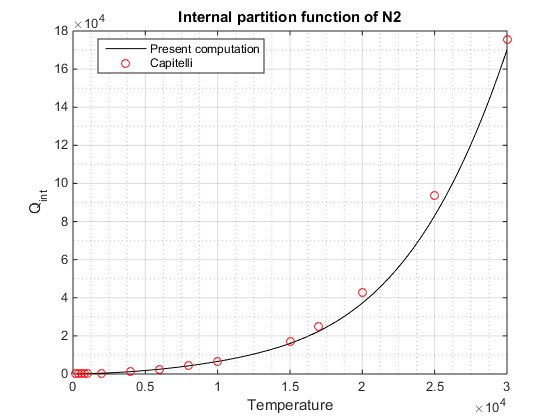
\includegraphics{QN2fig}
	\caption{From direct summation of approximated formula.}
\end{figure}


\begin{figure}[H!]% order of placement preference: here, top, bottom
	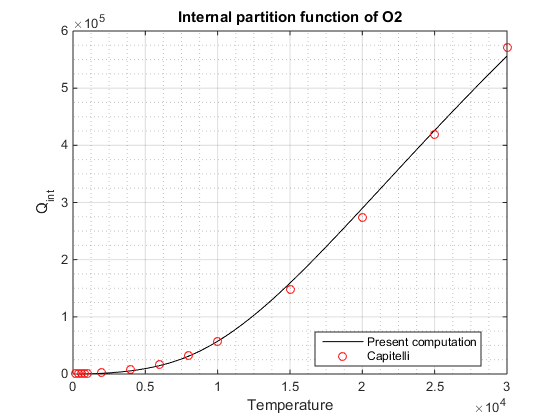
\includegraphics{QO2fig}
	\caption{From direct summation.}
\end{figure}


\subsection{Specific heat}

The variation of specific heats for Nitrogen and Oxygen are shown below. The variations in the partition functions amplify in Cp. 

\begin{figure}[h]% order of placement preference: here, top, bottom
	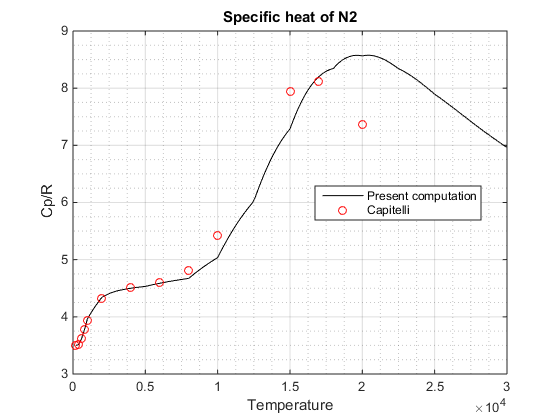
\includegraphics{CpN2fig}
	\caption{Using direct summation of approximated formula.}
\end{figure}


\begin{figure}[h]% order of placement preference: here, top, bottom
	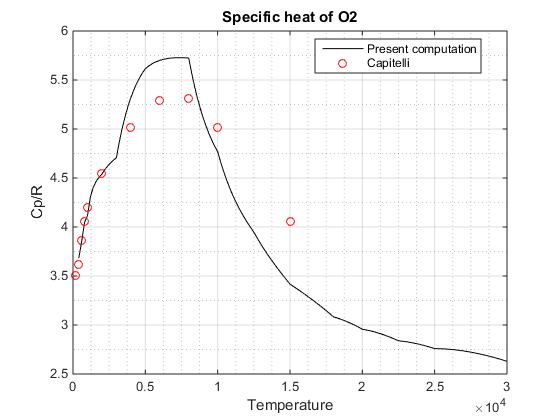
\includegraphics{CpO2fig}
	\caption{Using direct summation of approximated formula.}
\end{figure}


\subsection{Composition and equilibrium constant}

The variaton is again shown for Nitrogen and Oxygen. The comparison is done with Barklem \cite{Barklem:1}. 

\begin{figure}[h]% order of placement preference: here, top, bottom
	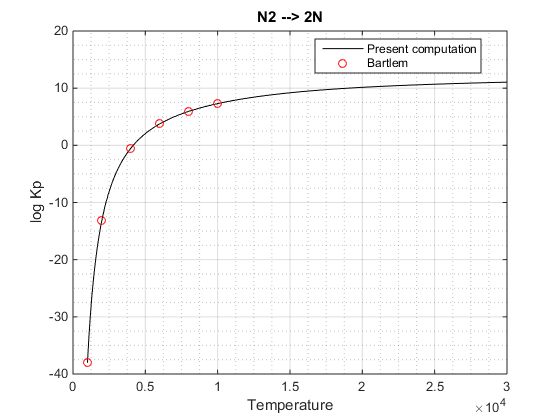
\includegraphics{KpN2fig}
	\caption{Using direct summation of approximated formula.}
	\end{figure}

\begin{figure}[h]% order of placement preference: here, top, bottom
	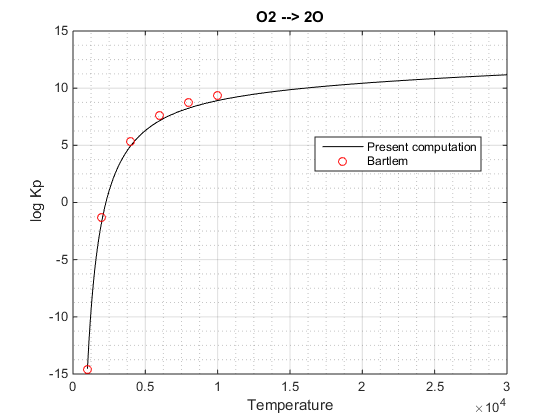
\includegraphics{KpO2fig}
	\caption{Using direct summation of approximated formula.}
	\end{figure}

\begin{figure}[h]% order of placement preference: here, top, bottom
	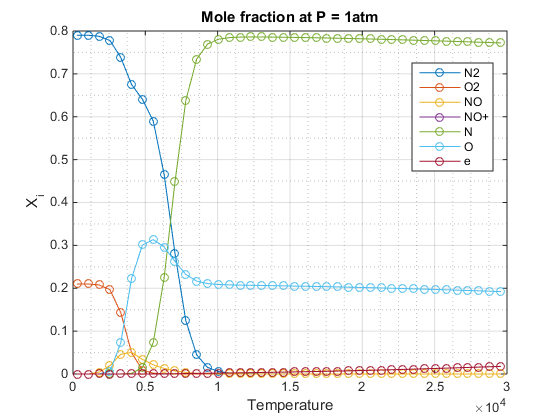
\includegraphics{comp1atmfig}
	\caption{It can be seen that the molar fraction of the charged species is much less than N and O. But the dissociation of Nitrogen and Oxygen is almost complete.}
	\end{figure}

\begin{figure}[h]% order of placement preference: here, top, bottom
	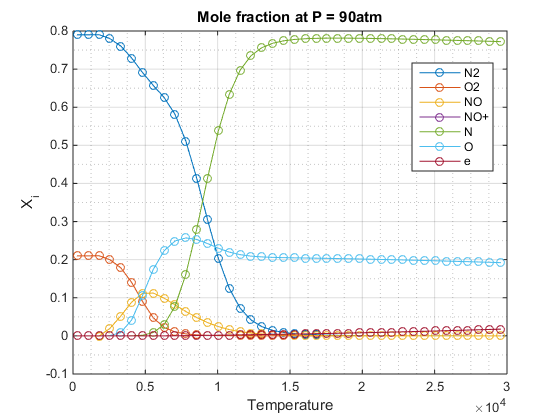
\includegraphics{comp90atmfig}
	\caption{The higher pressure suppresses dissociation as expected from the Le Chatelier's principle.}
	\end{figure}

\subsection{Mixture thermodynamic properties}

The thermodynamic properties of air are shown below. 

\begin{figure}[h]% order of placement preference: here, top, bottom
	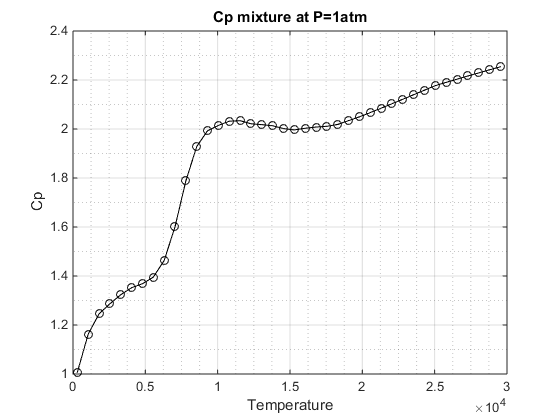
\includegraphics{Cpair1atmfig}
	\caption{Spline interpolated from spline interpolated partition function.}
	\end{figure}

\begin{figure}[h]% order of placement preference: here, top, bottom
	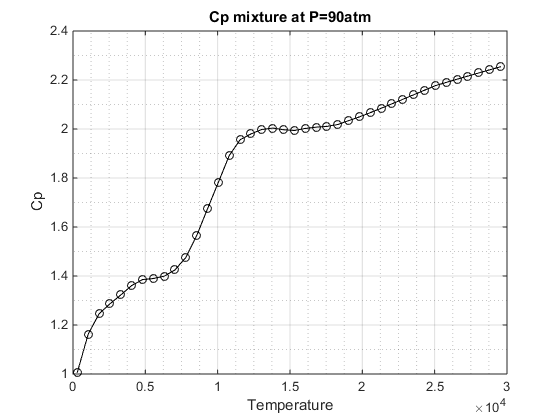
\includegraphics{Cpair90atmfig}
	\caption{Spline interpolated from spline interpolated partition function.}
	\end{figure}

\subsection{Curve fits}

Tabulated below are the curve fits for specific heat of Nitrogen. All the other tables are similar in nature.

\begin{table}% no placement specified: defaults to here, top, bottom, page
	\begin{center}
		\caption{Curve-fit for Cp/R of Nitrogen}
		\begin{tabular}{cccccc}
			Coefficients & 100K-2500K & 2500K-8000K & 8000K-18000K & 18000K-22000K & 22000K-30000K\\\hline
			A1 &  1.6637946e+00 &  3.1651973e-03 & -1.5047620e-04 & -1.0190640e-03 & -8.7801382e-04 \\
			A2 &  -2.4434158e+00 &  7.2433194e-04 & -6.8701167e-04 &  2.2599813e-03 &  1.1746039e-03\\
			A3 &  3.5623756e+00 & -2.5806735e-03 & -1.4242511e-03 &  7.3481886e-04 &  3.2102028e-04\\
			A4 & -6.5831490e-04 &  3.7917134e-03 &  1.9003863e-03 & -1.8408490e-03  & 1.1638909e-03\\
			A5 & 1.8386176e-06 & -1.1494748e-06 & -3.0988192e-07  & 3.5645687e-07 & -4.4102326e-08 \\
			A6 & -9.9656386e-10  & 1.4890337e-10  & 2.2491837e-11 & -1.7551239e-11  & 2.7304215e-13\\
			A7 &   1.6856875e-13 & -6.9215436e-15 & -5.3935701e-16  & 2.7018838e-16  & 5.3915305e-18 \\
		\end{tabular}
	\end{center}
\end{table}

\section{Conclusions and discussions}

This report apart from producing data pertaining to relevant thermodynamic parameters, more importantly has documented data of spectroscopic data and partition function data along with curve fits for air. This can come in handy to other enthusiasts. 

\begin{enumerate}
	\item The reason for an error of sometimes upto 10\% can be attributed to the fact that the electronic levels considered in computations such as these is a arbitrary.
	\item The cut-off criterion for some of the ions is based on the electronic energy decrement which is again taken as a parameter or arbitrarily fixed.
	\item Care has to be taken to verify that Jmax has converged for each iteration. This was unfortunately not done and could have contributed to some of the variation between this report and Capitelli's.
	\item A lot of the literature shows a wide range of values. The numbers got out of this report lie somewhere in between.
	\item Discrepancies arise mostly at temperatures greater than about 10000K. Most of the work done so far are upto 10000K. Results match closely up till that range. Only after does the uncertainty creep in.
\end{enumerate}

	


\section*{Acknowledgments}

I am thankful to Dr. Satheesh K. for providing such a rigorous assignment. I am grateful to my friend Mr. Pillai Anek Venudas for helping me type out some of the many equations in the report.


\begin{thebibliography}{9}% maximum number of references (for label width)

 \bibitem{Barklem:1}
 P.S Barklem and 	R. Collet. Partition functions and equilibrium constants for diatomic molecules and atoms of astrophysical interest, Astronomy and Astrophysics 588, A96 (2016)
 DOI: 10.1051/0004-6361/201526961
 
 \bibitem{Capitelli:1}
 Capitelli, Mario, et al., Tables of internal partition functions and thermodynamic properties of high-temperature
 mars-atmosphere species from 50k to 50000k, Vol. 246. 2005.
 
 \bibitem{Tatum:1}
 J. B. Tatum. Accurate partition functions and dissociation equilibrium constants of diatomic molecules of astrophysical interest, Dominion astrophysical observatory, Volume XIII, No.1, 1966.
 
 \bibitem{carlos:1}
 Carlos Alberto Rocha Pimentel and Annibal Hetem Jr. Computation of air chemical
 equilibrium composition until 30000K - Part I, doi: 10.5028/jatm.2011.03021011.
 
 \bibitem{mayer:2}
 Mayer, J. E., MG Mayer Statistical mechanics., (1940): 437.
 
 \bibitem{tanehill:1}
 S. Srinivasan, J. C. Tanehill and K. J. Weilmuenster. Simplified curve fits for the thermodynamic properties of equilibrium air. NASA Grant NAG-1-313, 1986.
 
 \bibitem{drellishak:1}
 Drellishak, K. S., D. P. Aeschliman, and Ali Bulent Cambel., Partition functions and thermodynamic properties of nitrogen
 and oxygen plasmas., The Physics of Fluids 8.9 (1965): 1590-1600.
 
 \bibitem{padman:1}
 Md. Sabir Alam et. al., High Temperature Gas Dynamics Assignment, Question 4, 2017.
 
\end{thebibliography}

\end{document}

% $Id: template_basic.tex,v 1.5 2004/05/23 12:49:44 kleb Exp $
